%
%  PACKAGE IMPORTS
%
\documentclass{article} % For LaTeX2e
\usepackage{iclr2022_conference,times}
%%%%% NEW MATH DEFINITIONS %%%%%

\usepackage{amsmath,amsfonts,bm}

% Mark sections of captions for referring to divisions of figures
\newcommand{\figleft}{{\em (Left)}}
\newcommand{\figcenter}{{\em (Center)}}
\newcommand{\figright}{{\em (Right)}}
\newcommand{\figtop}{{\em (Top)}}
\newcommand{\figbottom}{{\em (Bottom)}}
\newcommand{\captiona}{{\em (a)}}
\newcommand{\captionb}{{\em (b)}}
\newcommand{\captionc}{{\em (c)}}
\newcommand{\captiond}{{\em (d)}}

% Highlight a newly defined term
\newcommand{\newterm}[1]{{\bf #1}}


% Figure reference, lower-case.
\def\figref#1{figure~\ref{#1}}
% Figure reference, capital. For start of sentence
\def\Figref#1{Figure~\ref{#1}}
\def\twofigref#1#2{figures \ref{#1} and \ref{#2}}
\def\quadfigref#1#2#3#4{figures \ref{#1}, \ref{#2}, \ref{#3} and \ref{#4}}
% Section reference, lower-case.
\def\secref#1{section~\ref{#1}}
% Section reference, capital.
\def\Secref#1{Section~\ref{#1}}
% Reference to two sections.
\def\twosecrefs#1#2{sections \ref{#1} and \ref{#2}}
% Reference to three sections.
\def\secrefs#1#2#3{sections \ref{#1}, \ref{#2} and \ref{#3}}
% Reference to an equation, lower-case.
\def\eqref#1{equation~\ref{#1}}
% Reference to an equation, upper case
\def\Eqref#1{Equation~\ref{#1}}
% A raw reference to an equation---avoid using if possible
\def\plaineqref#1{\ref{#1}}
% Reference to a chapter, lower-case.
\def\chapref#1{chapter~\ref{#1}}
% Reference to an equation, upper case.
\def\Chapref#1{Chapter~\ref{#1}}
% Reference to a range of chapters
\def\rangechapref#1#2{chapters\ref{#1}--\ref{#2}}
% Reference to an algorithm, lower-case.
\def\algref#1{algorithm~\ref{#1}}
% Reference to an algorithm, upper case.
\def\Algref#1{Algorithm~\ref{#1}}
\def\twoalgref#1#2{algorithms \ref{#1} and \ref{#2}}
\def\Twoalgref#1#2{Algorithms \ref{#1} and \ref{#2}}
% Reference to a part, lower case
\def\partref#1{part~\ref{#1}}
% Reference to a part, upper case
\def\Partref#1{Part~\ref{#1}}
\def\twopartref#1#2{parts \ref{#1} and \ref{#2}}

\def\ceil#1{\lceil #1 \rceil}
\def\floor#1{\lfloor #1 \rfloor}
\def\1{\bm{1}}
\newcommand{\train}{\mathcal{D}}
\newcommand{\valid}{\mathcal{D_{\mathrm{valid}}}}
\newcommand{\test}{\mathcal{D_{\mathrm{test}}}}

\def\eps{{\epsilon}}


% Random variables
\def\reta{{\textnormal{$\eta$}}}
\def\ra{{\textnormal{a}}}
\def\rb{{\textnormal{b}}}
\def\rc{{\textnormal{c}}}
\def\rd{{\textnormal{d}}}
\def\re{{\textnormal{e}}}
\def\rf{{\textnormal{f}}}
\def\rg{{\textnormal{g}}}
\def\rh{{\textnormal{h}}}
\def\ri{{\textnormal{i}}}
\def\rj{{\textnormal{j}}}
\def\rk{{\textnormal{k}}}
\def\rl{{\textnormal{l}}}
% rm is already a command, just don't name any random variables m
\def\rn{{\textnormal{n}}}
\def\ro{{\textnormal{o}}}
\def\rp{{\textnormal{p}}}
\def\rq{{\textnormal{q}}}
\def\rr{{\textnormal{r}}}
\def\rs{{\textnormal{s}}}
\def\rt{{\textnormal{t}}}
\def\ru{{\textnormal{u}}}
\def\rv{{\textnormal{v}}}
\def\rw{{\textnormal{w}}}
\def\rx{{\textnormal{x}}}
\def\ry{{\textnormal{y}}}
\def\rz{{\textnormal{z}}}

% Random vectors
\def\rvepsilon{{\mathbf{\epsilon}}}
\def\rvtheta{{\mathbf{\theta}}}
\def\rva{{\mathbf{a}}}
\def\rvb{{\mathbf{b}}}
\def\rvc{{\mathbf{c}}}
\def\rvd{{\mathbf{d}}}
\def\rve{{\mathbf{e}}}
\def\rvf{{\mathbf{f}}}
\def\rvg{{\mathbf{g}}}
\def\rvh{{\mathbf{h}}}
\def\rvu{{\mathbf{i}}}
\def\rvj{{\mathbf{j}}}
\def\rvk{{\mathbf{k}}}
\def\rvl{{\mathbf{l}}}
\def\rvm{{\mathbf{m}}}
\def\rvn{{\mathbf{n}}}
\def\rvo{{\mathbf{o}}}
\def\rvp{{\mathbf{p}}}
\def\rvq{{\mathbf{q}}}
\def\rvr{{\mathbf{r}}}
\def\rvs{{\mathbf{s}}}
\def\rvt{{\mathbf{t}}}
\def\rvu{{\mathbf{u}}}
\def\rvv{{\mathbf{v}}}
\def\rvw{{\mathbf{w}}}
\def\rvx{{\mathbf{x}}}
\def\rvy{{\mathbf{y}}}
\def\rvz{{\mathbf{z}}}

% Elements of random vectors
\def\erva{{\textnormal{a}}}
\def\ervb{{\textnormal{b}}}
\def\ervc{{\textnormal{c}}}
\def\ervd{{\textnormal{d}}}
\def\erve{{\textnormal{e}}}
\def\ervf{{\textnormal{f}}}
\def\ervg{{\textnormal{g}}}
\def\ervh{{\textnormal{h}}}
\def\ervi{{\textnormal{i}}}
\def\ervj{{\textnormal{j}}}
\def\ervk{{\textnormal{k}}}
\def\ervl{{\textnormal{l}}}
\def\ervm{{\textnormal{m}}}
\def\ervn{{\textnormal{n}}}
\def\ervo{{\textnormal{o}}}
\def\ervp{{\textnormal{p}}}
\def\ervq{{\textnormal{q}}}
\def\ervr{{\textnormal{r}}}
\def\ervs{{\textnormal{s}}}
\def\ervt{{\textnormal{t}}}
\def\ervu{{\textnormal{u}}}
\def\ervv{{\textnormal{v}}}
\def\ervw{{\textnormal{w}}}
\def\ervx{{\textnormal{x}}}
\def\ervy{{\textnormal{y}}}
\def\ervz{{\textnormal{z}}}

% Random matrices
\def\rmA{{\mathbf{A}}}
\def\rmB{{\mathbf{B}}}
\def\rmC{{\mathbf{C}}}
\def\rmD{{\mathbf{D}}}
\def\rmE{{\mathbf{E}}}
\def\rmF{{\mathbf{F}}}
\def\rmG{{\mathbf{G}}}
\def\rmH{{\mathbf{H}}}
\def\rmI{{\mathbf{I}}}
\def\rmJ{{\mathbf{J}}}
\def\rmK{{\mathbf{K}}}
\def\rmL{{\mathbf{L}}}
\def\rmM{{\mathbf{M}}}
\def\rmN{{\mathbf{N}}}
\def\rmO{{\mathbf{O}}}
\def\rmP{{\mathbf{P}}}
\def\rmQ{{\mathbf{Q}}}
\def\rmR{{\mathbf{R}}}
\def\rmS{{\mathbf{S}}}
\def\rmT{{\mathbf{T}}}
\def\rmU{{\mathbf{U}}}
\def\rmV{{\mathbf{V}}}
\def\rmW{{\mathbf{W}}}
\def\rmX{{\mathbf{X}}}
\def\rmY{{\mathbf{Y}}}
\def\rmZ{{\mathbf{Z}}}

% Elements of random matrices
\def\ermA{{\textnormal{A}}}
\def\ermB{{\textnormal{B}}}
\def\ermC{{\textnormal{C}}}
\def\ermD{{\textnormal{D}}}
\def\ermE{{\textnormal{E}}}
\def\ermF{{\textnormal{F}}}
\def\ermG{{\textnormal{G}}}
\def\ermH{{\textnormal{H}}}
\def\ermI{{\textnormal{I}}}
\def\ermJ{{\textnormal{J}}}
\def\ermK{{\textnormal{K}}}
\def\ermL{{\textnormal{L}}}
\def\ermM{{\textnormal{M}}}
\def\ermN{{\textnormal{N}}}
\def\ermO{{\textnormal{O}}}
\def\ermP{{\textnormal{P}}}
\def\ermQ{{\textnormal{Q}}}
\def\ermR{{\textnormal{R}}}
\def\ermS{{\textnormal{S}}}
\def\ermT{{\textnormal{T}}}
\def\ermU{{\textnormal{U}}}
\def\ermV{{\textnormal{V}}}
\def\ermW{{\textnormal{W}}}
\def\ermX{{\textnormal{X}}}
\def\ermY{{\textnormal{Y}}}
\def\ermZ{{\textnormal{Z}}}

% Vectors
\def\vzero{{\bm{0}}}
\def\vone{{\bm{1}}}
\def\vmu{{\bm{\mu}}}
\def\vtheta{{\bm{\theta}}}
\def\va{{\bm{a}}}
\def\vb{{\bm{b}}}
\def\vc{{\bm{c}}}
\def\vd{{\bm{d}}}
\def\ve{{\bm{e}}}
\def\vf{{\bm{f}}}
\def\vg{{\bm{g}}}
\def\vh{{\bm{h}}}
\def\vi{{\bm{i}}}
\def\vj{{\bm{j}}}
\def\vk{{\bm{k}}}
\def\vl{{\bm{l}}}
\def\vm{{\bm{m}}}
\def\vn{{\bm{n}}}
\def\vo{{\bm{o}}}
\def\vp{{\bm{p}}}
\def\vq{{\bm{q}}}
\def\vr{{\bm{r}}}
\def\vs{{\bm{s}}}
\def\vt{{\bm{t}}}
\def\vu{{\bm{u}}}
\def\vv{{\bm{v}}}
\def\vw{{\bm{w}}}
\def\vx{{\bm{x}}}
\def\vy{{\bm{y}}}
\def\vz{{\bm{z}}}

% Elements of vectors
\def\evalpha{{\alpha}}
\def\evbeta{{\beta}}
\def\evepsilon{{\epsilon}}
\def\evlambda{{\lambda}}
\def\evomega{{\omega}}
\def\evmu{{\mu}}
\def\evpsi{{\psi}}
\def\evsigma{{\sigma}}
\def\evtheta{{\theta}}
\def\eva{{a}}
\def\evb{{b}}
\def\evc{{c}}
\def\evd{{d}}
\def\eve{{e}}
\def\evf{{f}}
\def\evg{{g}}
\def\evh{{h}}
\def\evi{{i}}
\def\evj{{j}}
\def\evk{{k}}
\def\evl{{l}}
\def\evm{{m}}
\def\evn{{n}}
\def\evo{{o}}
\def\evp{{p}}
\def\evq{{q}}
\def\evr{{r}}
\def\evs{{s}}
\def\evt{{t}}
\def\evu{{u}}
\def\evv{{v}}
\def\evw{{w}}
\def\evx{{x}}
\def\evy{{y}}
\def\evz{{z}}

% Matrix
\def\mA{{\bm{A}}}
\def\mB{{\bm{B}}}
\def\mC{{\bm{C}}}
\def\mD{{\bm{D}}}
\def\mE{{\bm{E}}}
\def\mF{{\bm{F}}}
\def\mG{{\bm{G}}}
\def\mH{{\bm{H}}}
\def\mI{{\bm{I}}}
\def\mJ{{\bm{J}}}
\def\mK{{\bm{K}}}
\def\mL{{\bm{L}}}
\def\mM{{\bm{M}}}
\def\mN{{\bm{N}}}
\def\mO{{\bm{O}}}
\def\mP{{\bm{P}}}
\def\mQ{{\bm{Q}}}
\def\mR{{\bm{R}}}
\def\mS{{\bm{S}}}
\def\mT{{\bm{T}}}
\def\mU{{\bm{U}}}
\def\mV{{\bm{V}}}
\def\mW{{\bm{W}}}
\def\mX{{\bm{X}}}
\def\mY{{\bm{Y}}}
\def\mZ{{\bm{Z}}}
\def\mBeta{{\bm{\beta}}}
\def\mPhi{{\bm{\Phi}}}
\def\mLambda{{\bm{\Lambda}}}
\def\mSigma{{\bm{\Sigma}}}

% Tensor
\DeclareMathAlphabet{\mathsfit}{\encodingdefault}{\sfdefault}{m}{sl}
\SetMathAlphabet{\mathsfit}{bold}{\encodingdefault}{\sfdefault}{bx}{n}
\newcommand{\tens}[1]{\bm{\mathsfit{#1}}}
\def\tA{{\tens{A}}}
\def\tB{{\tens{B}}}
\def\tC{{\tens{C}}}
\def\tD{{\tens{D}}}
\def\tE{{\tens{E}}}
\def\tF{{\tens{F}}}
\def\tG{{\tens{G}}}
\def\tH{{\tens{H}}}
\def\tI{{\tens{I}}}
\def\tJ{{\tens{J}}}
\def\tK{{\tens{K}}}
\def\tL{{\tens{L}}}
\def\tM{{\tens{M}}}
\def\tN{{\tens{N}}}
\def\tO{{\tens{O}}}
\def\tP{{\tens{P}}}
\def\tQ{{\tens{Q}}}
\def\tR{{\tens{R}}}
\def\tS{{\tens{S}}}
\def\tT{{\tens{T}}}
\def\tU{{\tens{U}}}
\def\tV{{\tens{V}}}
\def\tW{{\tens{W}}}
\def\tX{{\tens{X}}}
\def\tY{{\tens{Y}}}
\def\tZ{{\tens{Z}}}


% Graph
\def\gA{{\mathcal{A}}}
\def\gB{{\mathcal{B}}}
\def\gC{{\mathcal{C}}}
\def\gD{{\mathcal{D}}}
\def\gE{{\mathcal{E}}}
\def\gF{{\mathcal{F}}}
\def\gG{{\mathcal{G}}}
\def\gH{{\mathcal{H}}}
\def\gI{{\mathcal{I}}}
\def\gJ{{\mathcal{J}}}
\def\gK{{\mathcal{K}}}
\def\gL{{\mathcal{L}}}
\def\gM{{\mathcal{M}}}
\def\gN{{\mathcal{N}}}
\def\gO{{\mathcal{O}}}
\def\gP{{\mathcal{P}}}
\def\gQ{{\mathcal{Q}}}
\def\gR{{\mathcal{R}}}
\def\gS{{\mathcal{S}}}
\def\gT{{\mathcal{T}}}
\def\gU{{\mathcal{U}}}
\def\gV{{\mathcal{V}}}
\def\gW{{\mathcal{W}}}
\def\gX{{\mathcal{X}}}
\def\gY{{\mathcal{Y}}}
\def\gZ{{\mathcal{Z}}}

% Sets
\def\sA{{\mathbb{A}}}
\def\sB{{\mathbb{B}}}
\def\sC{{\mathbb{C}}}
\def\sD{{\mathbb{D}}}
% Don't use a set called E, because this would be the same as our symbol
% for expectation.
\def\sF{{\mathbb{F}}}
\def\sG{{\mathbb{G}}}
\def\sH{{\mathbb{H}}}
\def\sI{{\mathbb{I}}}
\def\sJ{{\mathbb{J}}}
\def\sK{{\mathbb{K}}}
\def\sL{{\mathbb{L}}}
\def\sM{{\mathbb{M}}}
\def\sN{{\mathbb{N}}}
\def\sO{{\mathbb{O}}}
\def\sP{{\mathbb{P}}}
\def\sQ{{\mathbb{Q}}}
\def\sR{{\mathbb{R}}}
\def\sS{{\mathbb{S}}}
\def\sT{{\mathbb{T}}}
\def\sU{{\mathbb{U}}}
\def\sV{{\mathbb{V}}}
\def\sW{{\mathbb{W}}}
\def\sX{{\mathbb{X}}}
\def\sY{{\mathbb{Y}}}
\def\sZ{{\mathbb{Z}}}

% Entries of a matrix
\def\emLambda{{\Lambda}}
\def\emA{{A}}
\def\emB{{B}}
\def\emC{{C}}
\def\emD{{D}}
\def\emE{{E}}
\def\emF{{F}}
\def\emG{{G}}
\def\emH{{H}}
\def\emI{{I}}
\def\emJ{{J}}
\def\emK{{K}}
\def\emL{{L}}
\def\emM{{M}}
\def\emN{{N}}
\def\emO{{O}}
\def\emP{{P}}
\def\emQ{{Q}}
\def\emR{{R}}
\def\emS{{S}}
\def\emT{{T}}
\def\emU{{U}}
\def\emV{{V}}
\def\emW{{W}}
\def\emX{{X}}
\def\emY{{Y}}
\def\emZ{{Z}}
\def\emSigma{{\Sigma}}

% entries of a tensor
% Same font as tensor, without \bm wrapper
\newcommand{\etens}[1]{\mathsfit{#1}}
\def\etLambda{{\etens{\Lambda}}}
\def\etA{{\etens{A}}}
\def\etB{{\etens{B}}}
\def\etC{{\etens{C}}}
\def\etD{{\etens{D}}}
\def\etE{{\etens{E}}}
\def\etF{{\etens{F}}}
\def\etG{{\etens{G}}}
\def\etH{{\etens{H}}}
\def\etI{{\etens{I}}}
\def\etJ{{\etens{J}}}
\def\etK{{\etens{K}}}
\def\etL{{\etens{L}}}
\def\etM{{\etens{M}}}
\def\etN{{\etens{N}}}
\def\etO{{\etens{O}}}
\def\etP{{\etens{P}}}
\def\etQ{{\etens{Q}}}
\def\etR{{\etens{R}}}
\def\etS{{\etens{S}}}
\def\etT{{\etens{T}}}
\def\etU{{\etens{U}}}
\def\etV{{\etens{V}}}
\def\etW{{\etens{W}}}
\def\etX{{\etens{X}}}
\def\etY{{\etens{Y}}}
\def\etZ{{\etens{Z}}}

% The true underlying data generating distribution
\newcommand{\pdata}{p_{\rm{data}}}
% The empirical distribution defined by the training set
\newcommand{\ptrain}{\hat{p}_{\rm{data}}}
\newcommand{\Ptrain}{\hat{P}_{\rm{data}}}
% The model distribution
\newcommand{\pmodel}{p_{\rm{model}}}
\newcommand{\Pmodel}{P_{\rm{model}}}
\newcommand{\ptildemodel}{\tilde{p}_{\rm{model}}}
% Stochastic autoencoder distributions
\newcommand{\pencode}{p_{\rm{encoder}}}
\newcommand{\pdecode}{p_{\rm{decoder}}}
\newcommand{\precons}{p_{\rm{reconstruct}}}

\newcommand{\laplace}{\mathrm{Laplace}} % Laplace distribution

\newcommand{\E}{\mathbb{E}}
\newcommand{\Ls}{\mathcal{L}}
\newcommand{\R}{\mathbb{R}}
\newcommand{\emp}{\tilde{p}}
\newcommand{\lr}{\alpha}
\newcommand{\reg}{\lambda}
\newcommand{\rect}{\mathrm{rectifier}}
\newcommand{\softmax}{\mathrm{softmax}}
\newcommand{\sigmoid}{\sigma}
\newcommand{\softplus}{\zeta}
\newcommand{\KL}{D_{\mathrm{KL}}}
\newcommand{\Var}{\mathrm{Var}}
\newcommand{\standarderror}{\mathrm{SE}}
\newcommand{\Cov}{\mathrm{Cov}}
% Wolfram Mathworld says $L^2$ is for function spaces and $\ell^2$ is for vectors
% But then they seem to use $L^2$ for vectors throughout the site, and so does
% wikipedia.
\newcommand{\normlzero}{L^0}
\newcommand{\normlone}{L^1}
\newcommand{\normltwo}{L^2}
\newcommand{\normlp}{L^p}
\newcommand{\normmax}{L^\infty}

\newcommand{\parents}{Pa} % See usage in notation.tex. Chosen to match Daphne's book.

\DeclareMathOperator*{\argmax}{arg\,max}
\DeclareMathOperator*{\argmin}{arg\,min}

\DeclareMathOperator{\sign}{sign}
\DeclareMathOperator{\Tr}{Tr}
\let\ab\allowbreak


\newcommand{\apsname}{Project Proposal}
\newcommand{\gpnumber}{26}

\usepackage{hyperref}
\usepackage{url}
\usepackage{graphicx}
\usepackage[table]{xcolor}

\usepackage{graphicx} % Required for \resizebox
\usepackage{placeins} % Required for \FloatBarrier

%
%  TITLE AND AUTHORS
%
\title{Deep learning approach to  \\ 
mushroom species classification}

\author{Yanni Alan Alevras  \\
Student\# 1009330706 \\
\texttt{yanni.alevras@mail.utoronto.ca} \\
\And
Nicholas Biancolin  \\
Student\# 1005678901 \\
\texttt{n.biancolin@mail.utoronto.ca} \\
\AND
Eric Liu  \\
Student\# 1009098450 \\
\texttt{ey.liu@mail.utoronto.ca} \\
\And
Jason Ruixuan Zhang \\
Student\# 1008997631 \\
\texttt{jasonrx.zhang@mail.utoronto.ca} \\
\AND
}

\newcommand{\fix}{\marginpar{FIX}}
\newcommand{\new}{\marginpar{NEW}}

\iclrfinalcopy

%
%   DOCUMENT STARTS HERE
%
\begin{document}
\maketitle

\section{Introduction}
\label{intro}

The format for the submissions is a variant of the ICLR 2022 format.
Please read carefully the instructions below, and follow them
faithfully. There is a \textbf{9 page} limit for the main text. References do not have any limitation. This is also ICLR's standard length for a paper submission. 
If your main text goes to page 10,a a $-20\%$ penalty would be applied. If your main text goes to page 11, you will not receive any grade for your submission. 

We propose the use of the MIND.Funga dataset \citep{Drechsler-SantosKarstedtEtAl.MINDFunga.2023}, which has approximately 17 000 images of nearly 500 species of fungi. This dataset is well-suited for our project, as it is built primarily for use in deep classification models. Images are also curated to be of a high quality and are labelled by species.

Our code can be found at this \href{https://github.com/nbiancolin/convolutional-neural-nuts}{GitHub repository}.

\section{Background \& Related Work}
\label{bg_related}

One key application of a fungi identification model is food safety and satisfaction.

In Bangladesh, a country with a large mushroom production, a farming method was developed by \cite{RahmanFaruqEtAl.IoTEnabledMushroom.2022} using machine learning to classify which mushrooms are being harvested. This system intended to remove toxic species that may have grown in the same area as the target mushroom. \cite{WangZhengEtAl.AutomaticSortingSystem.2018} created an algorithm to identify disease, discolouration, freshness, as well as other factors contributing to the commercial quality of a white button mushroom.

Our software would sort these mushrooms into genera, which would assist in identifying different types of mushrooms instead of certain physical features. Keeping with the theme of food quality, in Taiwan, \cite{LuLiawEtAl.DevelopmentMushroomGrowth.2019} developed a system to determine how much a mushroom has grown using an image recognition model, which produces an estimate based on images from different times. This used a convolutional neural network (CNN) to provide these results, which will be similar to our model's architecture. In the Chinese province of Yunnan, \cite{H.ZhaoF.GeEtAl.IdentificationWildMushroom.2021} created a wild mushroom identification model that used a CNN to identify edible and medicinal mushrooms due to increasing popular interest in mushrooms.

Other field work includes smartphone applications for recreational use, like ShroomID, which details mushroom species, while providing a heatmap of its location and seasonality. This educational tool provides useful information about a mushroom, after it has been identified using a classification model \citep{.ShroomID.2023}.

\section{Data Processing}
\label{data}

Many species in the dataset have a relatively small amount of images associated with them ($<30$ images), which may be detrimental when training, testing, and validating our model. To mitigate this, we intend to group images into larger “buckets” corresponding to a higher level of taxonomic classification, i.e., grouping by genus instead of by species. This is a simple way to reduce the number of classes our model must be trained on, and to increase the amount of data to a sufficient amount that model features can be reasonably trained. Genera form an ideal way to group images together — biologically species of the same genus share many physical characteristics, and they share a root name (the first word in the species name), which enhances ease of processing. Existing literature \citep{HollisterCaiEtAl.UsingComputerVision.2023} also suggests that models trained to classify genera tend to have better accuracy and are less difficult to train than species-level classification.

Once we have performed this combination, any genera with less than 75 images will be discarded from the dataset. This matches the lower threshold of published ecological classifiers, like iNaturalist \citep{Shepard.LatestComputerVision.2022} or models trained on the ETHZ human dataset \citep{SchneiderTaylorEtAl.PresentFutureApproaches.2019}. It also matches what is considered by \cite{FarleyMehrotaEtAl.ImprovingYourModel.2024} to be the lower end of images per class to train a model without overfitting.

\section{Architecture}
Since our project primarily involves images, we plan to follow a workflow similar to that described by \cite{S.RenK.HeEtAl.FasterRCNNRealTime.2017}. We will first apply a regional proposal network (RPN) that first isolates the macrofungi from the image. RPNs are convolutional networks that are able to identify regions of interest (proposals) in an image.

We will then apply a convolutional neural network (CNN) for detection and identification training. Prior literature \citep{BarreStoverEtAl.LeafNetComputerVision.2017} suggests that a CNN is best suited for computer vision classification problems, especially in ecology-related settings.

We also intend to use a stochastic gradient descent-based optimizer, as it is a common choice for training deep neural networks \citep{JamesWittenEtAl.IntroductionStatisticalLearning.2023}.

\begin{figure}[h]
  \begin{center}
  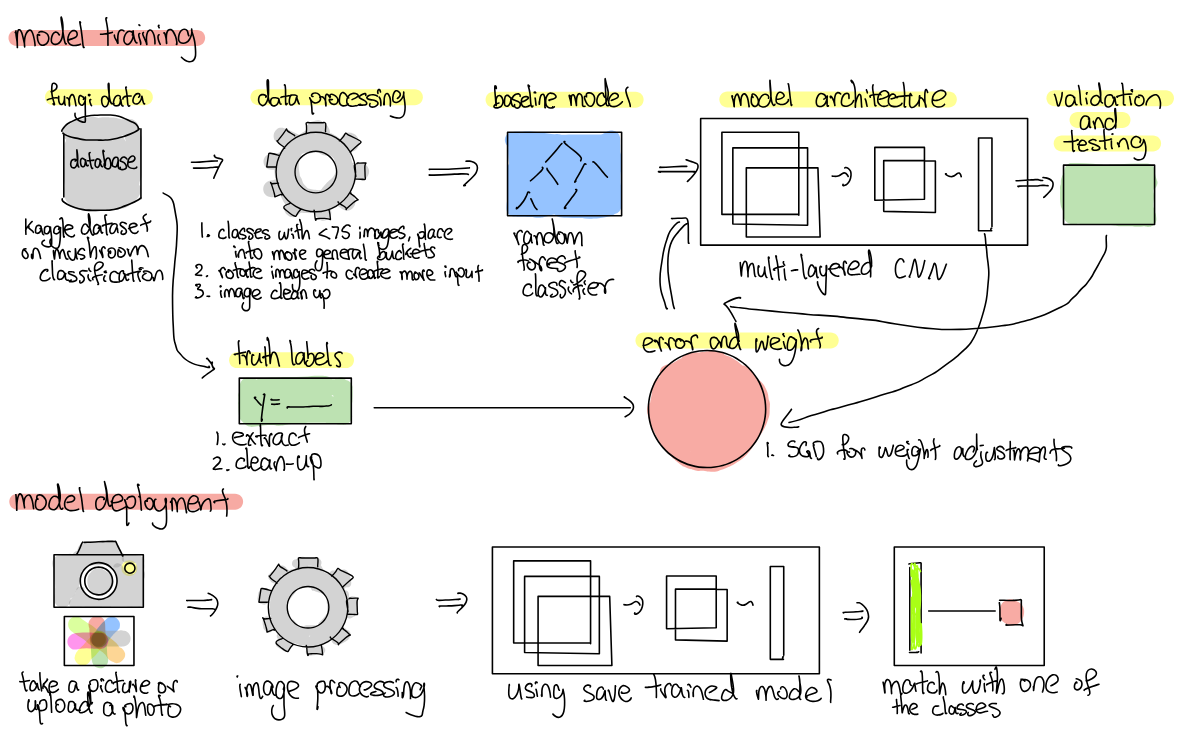
\includegraphics[width=0.6\textwidth]{figures/model.png}
  \end{center}
  \caption{Proposed model training and deployment pipeline}
\end{figure}

\section{Baseline Model}
For the baseline model we are comparing our model against, we selected a random forest classifier model. Our goal is to identify several hundred species of macrofungi, making this a multiclass classification problem. Decision trees like random forest are generally suited for multiclass problems \citep{GallRazaviEtAl.IntroductionRandomForests.2012}. Other methods, like support vector machines, are generally suitable primarily for binary classification problems \citep{JamesWittenEtAl.IntroductionStatisticalLearning.2023}. 

We will compare the classification accuracy and training time for both models. The random forest model will be trained using the scikit-learn library with the same data and data processing steps as the neural network model, following the steps outlined in \cite{Shafl.RandomForestClassification.2023}.

\section{Project Plan}
Task Breakdown and Responsibilities (Green = completed, Yellow = in progress, Red = not started)\\
W = wrote/coded/drawn, ED = edited, MR = major revision, FP = Final section proofread

\begin{table}[ht]
    \centering
    \resizebox{\textwidth}{!}{%
    \begin{tabular}{|l|c|c|c|c|}
        \hline
        \rowcolor{gray!50}
        \textbf{Project Proposal} & \textbf{Eric Liu} & \textbf{Jason Zhang} & \textbf{Nicholas Biancolin} & \textbf{Yanni Alevras} \\
        \hline
        \rowcolor{green!50}
        Introduction (June 4th, 11:59pm) & W & W & W ED & W \\
        \hline
        \rowcolor{green!50}
        Illustration/Figure (June 5th 11:59pm) & W & ED & & \\
        \hline
        \rowcolor{green!50}
        Background and Related Work (June 5th 11:59pm) & & ED & & W \\
        \hline
        \rowcolor{green!50}
        Data Processing (June 5th 11:59pm) & & W & & \\
        \hline
        \rowcolor{green!50}
        Architecture (June 5th 11:59pm) & ED & W & & \\
        \hline
        \rowcolor{green!50}
        Baseline Model (June 5th 11:59pm) & ED & ED & W & \\
        \hline
        \rowcolor{green!50}
        Ethical Considerations (June 5th 11:59pm) & & & ED & W \\
        \hline
        \rowcolor{green!50}
        Project Plan (June 5th 11:59pm) & W & & & \\
        \hline
        \rowcolor{green!50}
        Task research and distribution (June 5th 11:59pm) & W & & & \\
        \hline
        \rowcolor{green!50}
        Risk Register (June 5th 11:59pm) & & & W & \\
        \hline
        \rowcolor{green!50}
        Github, References (June 5th 11:59pm) & ED & W & W & W\\
        \hline
        \rowcolor{green!50}
        Structure, Grammar and Mechanics (June 5th 11:59pm) & ED & W & & \\
        \hline
        \rowcolor{green!50}
        Document in LaTeX (June 5th 11:59pm) & W & W MR ED& & \\
        \hline
        \rowcolor{green!50}
        Editing (June 6th 11:59pm) & ED & ED & & \\
        \hline
        \rowcolor{green!50}
        Final Document Proofread (June 6th 11:59pm) & ED & ED & & \\
        \hline
    \end{tabular}}
    \caption{Project Proposal Task Breakdown}
\end{table}

\FloatBarrier


\begin{table}[ht]
    \centering
    \resizebox{\textwidth}{!}{%
    \begin{tabular}{|l|c|c|c|c|}
        \hline
        \rowcolor{gray!50}
        \textbf{Project Progress Report} & \textbf{Eric Liu} & \textbf{Jason Zhang} & \textbf{Nicholas Biancolin} & \textbf{Yanni Alevras} \\
        \hline
        \rowcolor{red!50}
        Brief Project Description (June 30th, 11:59 pm) & W & W & W & W\\
        \hline
        \rowcolor{red!50}
        Individual Contributions and Responsibilities (June 30th, 11:59 pm) & W & ED & & \\
        \hline
        \rowcolor{red!50}
        Contributions - Data Processing (June 30th, 11:59 pm) & & W & ED & \\
        \hline
        \rowcolor{red!50}
        Contributions - Baseline Model (June 30th, 11:59 pm) & & & W & ED\\
        \hline
        \rowcolor{red!50}
        Contributions - Primary Model (June 30th, 11:59 pm) & ED & & & W \\
        \hline
        \rowcolor{red!50}
        Illustrations (July 1st, 11:59 pm) & W & ED & & \\
        \hline
        \rowcolor{red!50}
        Latex format (July 2nd, 11:59 pm) & W & W & & \\
        \hline
        \rowcolor{red!50}
        Editing (July 3rd, 11:59 pm) & ED & ED & ED & ED\\
        \hline
        \rowcolor{red!50}
        Final Proofread (July 4th, 6:00 pm) & W & W & W & W \\
        \hline
    \end{tabular}}
    \caption{Project Progress Report Task Breakdown}
\end{table}

\FloatBarrier

\begin{table}[ht]
    \centering
    \resizebox{\textwidth}{!}{%
    \begin{tabular}{|l|c|c|c|c|}
        \hline
        \rowcolor{gray!50}
        \textbf{Project - Training and Testing} & \textbf{Eric Liu} & \textbf{Jason Zhang} & \textbf{Nicholas Biancolin} & \textbf{Yanni Alevras} \\
        \hline
        \rowcolor{red!50}
        In charge of code connection/solving merge conflicts (August 10th, 11:59pm) & & & & \\
        \hline
        \rowcolor{red!50}
        Data Cleaning (June 16th, 11:59pm) & & & & \\
        \hline
        \rowcolor{red!50}
        Image Grouping (June 16th, 11:59pm) & & & & \\
        \hline
        \rowcolor{red!50}
        Transfer data to training format (June 16th, 11:59pm) & & & & \\
        \hline
        \rowcolor{red!50}
        Data annotations, splitting (June 16th, 11:59pm) & & & & \\
        \hline
        \rowcolor{red!50}
        Model implementation (June 19th, 11:59pm) & & & & \\
        \hline
        \rowcolor{red!50}
        CNN architecture (June 19th, 11:59pm) & & & & \\
        \hline
        \rowcolor{red!50}
        Training Loop (June 19th, 11:59pm) & & & & \\
        \hline
        \rowcolor{red!50}
        Hyperparameter adjustments (July 15th, 11:59pm) & & & & \\
        \hline
        \rowcolor{red!50}
        Training (July 15th, 11:59pm) & & & & \\
        \hline
        \rowcolor{red!50}
        Validation (July 15th, 11:59pm) & & & & \\
        \hline
        \rowcolor{red!50}
        Testing (August 10th, 11:59pm) & & & & \\
        \hline
        \rowcolor{red!50}
        Iterative (if needed) (August 10th, 11:59pm) & & & & \\
        \hline
        \rowcolor{red!50}
        Evaluation (August 10th, 11:59pm) & & & & \\
        \hline
        \rowcolor{red!50}
        Documentation (August 10th, 11:59pm) & & & & \\
        \hline
        \rowcolor{red!50}
        Resource management (August 3rd, 11:59pm) & & & & \\
        \hline
        \rowcolor{red!50}
        Analyze Result for Presentation and Project (August 3rd, 11:59pm) & & & & \\
        \hline
    \end{tabular}}
    \caption{Project Training and Testing Task Breakdown}
\end{table}

\FloatBarrier

\begin{table}[ht]
    \centering
    \resizebox{\textwidth}{!}{%
    \begin{tabular}{|l|c|c|c|c|}
        \hline
        \rowcolor{gray!50}
        \textbf{Presentation} & \textbf{Eric Liu} & \textbf{Jason Zhang} & \textbf{Nicholas Biancolin} & \textbf{Yanni Alevras} \\
        \hline
        \rowcolor{red!50}
        Presentation Brainstorm (August 5th, 11:59pm) & & & & \\
        \hline
        \rowcolor{red!50}
        Problem - slides (August 5th, 11:59pm) & & & & \\
        \hline
        \rowcolor{red!50}
        Data Processing - slides (August 5th, 11:59pm) & & & & \\
        \hline
        \rowcolor{red!50}
        Model - slides (August 5th, 11:59pm) & & & & \\
        \hline
        \rowcolor{red!50}
        Result - slides (August 5th, 11:59pm) & & & & \\
        \hline
        \rowcolor{red!50}
        Slides Editing (August 5th, 11:59pm) & & & & \\
        \hline
        \rowcolor{red!50}
        Individual Practice (August 7th, 11:59pm) & & & & \\
        \hline
        \rowcolor{red!50}
        Group Practice (August 7th, 11:59pm) & & & & \\
        \hline
        \rowcolor{red!50}
        Record Presentation (August 7th, 11:59pm) & & & & \\
        \hline
        \rowcolor{red!50}
        Editing (August 10th, 11:59pm) & & & & \\
        \hline
    \end{tabular}}
    \caption{Presentation Task Breakdown}
\end{table}

\FloatBarrier

\begin{table}[ht]
    \centering
    \resizebox{\textwidth}{!}{%
    \begin{tabular}{|l|c|c|c|c|}
        \hline
        \rowcolor{gray!50}
        \textbf{Project Final Report} & \textbf{Eric Liu} & \textbf{Jason Zhang} & \textbf{Nicholas Biancolin} & \textbf{Yanni Alevras} \\
        \hline
        \rowcolor{red!50}
        Latex Formatting (August 12th, 11:59pm) & & & & \\
        \hline
        \rowcolor{red!50}
        Introduction (August 7th, 11:59pm) & & & & \\
        \hline
        \rowcolor{red!50}
        Illustration (August 7th, 11:59pm) & & & & \\
        \hline
        \rowcolor{red!50}
        Background and Related Work (August 7th, 11:59pm) & & & & \\
        \hline
        \rowcolor{red!50}
        Data Processing (August 7th, 11:59pm) & & & & \\
        \hline
        \rowcolor{red!50}
        Architecture (August 7th, 11:59pm) & & & & \\
        \hline
        \rowcolor{red!50}
        Baseline Model (August 7th, 11:59pm) & & & & \\
        \hline
        \rowcolor{red!50}
        Qualitative Results (August 7th, 11:59pm) & & & & \\
        \hline
        \rowcolor{red!50}
        Quantitative Results (August 7th, 11:59pm) & & & & \\
        \hline
        \rowcolor{red!50}
        Evaluation of Model (August 7th, 11:59pm) & & & & \\
        \hline
        \rowcolor{red!50}
        Discussion (August 7th, 11:59pm) & & & & \\
        \hline
        \rowcolor{red!50}
        Ethical Considerations (August 7th, 11:59pm) & & & & \\
        \hline
        \rowcolor{red!50}
        Project Difficulty (August 7th, 11:59pm) & & & & \\
        \hline
        \rowcolor{red!50}
        Editing (August 12th, 11:59pm) & & & & \\
        \hline
        \rowcolor{red!50}
        Final Proofread (August 14th, 11:59pm) & & & & \\
        \hline
    \end{tabular}}
    \caption{Project Final Report Task Breakdown}
\end{table}

\FloatBarrier

Note: The tasks and their assignments may change, particularly when a major task requires splitting into smaller more feasible ones. 

We (the team) plan to tackle all the tasks listed in the table above individually, as all tasks are planned out and distributed individually with clear deadlines. If any member cannot complete their task(s) on time, they must inform the team at the earliest convenience. A team meeting will then be held to determine whether to reassign the task, extend the deadline, or remove the task if it is of low priority. Given the team’s extensive experience working with each other, we (the team) have gained mutual trust and can resolve any potential issues together.

Coding tasks have been distributed so members will work on completely different sections, then push their functions into the main program. In addition, there is a member in charge of function integration and solving merge conflicts to ensure we will not write over each other's code.

We (the team) aim to meet at least twice a week via Discord calls, where the team discusses progress, tackles issues, and brainstorms ideas. The current meeting time is Wednesday and Saturday at 9 pm (Eastern Time), though this may change in the future. Our team's main source of communication will be Discord, and all members will check and reply to messages at least once every 12 hours.


\section{Risk Register}
As with any large scale project, there are many associated risks:

\begin{itemize}
  \item What if a team member elects to drop the course?
  \item What if the model isn't training properly?
  \item What happens if there's scope creep?
  \item What happens during time crunches?
\end{itemize}

We are privileged to have been friends for over a year. We have respect for and have worked with each other in the past. We recognise that a group member dropping the course, while far from ideal, is a choice that is made for a reason. Should such a case occur, we will meet and discuss how extra work will be divided and make a plan to ensure the project continues as planned with an extra workload.

We intend to avoid quality issues with the model by setting a timeline that leaves time for multiple rounds of iteration, further training, and debugging. If the model's performance is subpar, we intend to first make changes to the data processing and architecture. With a relatively small amount of data per class, deliberate improvements to both areas may be able to immediately improve performance.

As with many projects, this proposal was written with the understanding that circumstances may change as the semester continues. If left unchecked, project requirements can change drastically from the original proposal. We will keep this in mind as we discuss and work on the project to avoid any misconceptions.

Finally, we have experienced many short time constraints in previous projects and understand how they may affect the quality of the final product. The timeline we intend to set leaves extra room for unexpected issues. Should a time crunch occur, we will evaluate our responsibilities and progress and work according to a priority queue.

\label{last_page}

\bibliography{proposal_ref}
\bibliographystyle{iclr2022_conference}

\end{document}
